\section{Introduction}
% a contextual description of the goals of experiment


The detection of {\it exolife} is one of the most important goals for
future space missions. Current space missions used to identify exoplanets
include \texttt{COROT}, \texttt{Spitzer} and \texttt{the Hubble Space
Telescope}, as well as the secondary extended mission of \texttt{Deep Impact
(EPOCh)} which will observe the light reflected from exoplanets
\cite{arnold_etal07}. \texttt{ESA’s Darwin} mission (estimated launch 2015)
will aim to find and study the properties and composition of Earth-like
exoplanets in the infrared. Over 300 giant exoplanets already have been
detected, and hundreds, perhaps thousands more, are anticipated in the coming
years. The nature of these planets, including their orbits, masses, sizes,
constituents, and likelihood that life could develop on them, can be probed by a
combination of observations and modeling.

Our observations tie in with current and future missions to observe and
search for life on exoplanets. By looking at the spectra of Earth, we can
characterize what makes it suitable for sustaining life - information that can
be related to present and future exoplanet observations. This search is
characterized by the detection of possible {\it biomarkers} on Earth-like
exoplanets. On a first approach, they are simple molecules present in the
planet's atmosphere, such as $O_2, O_3, CO_2,$ and $H_2O$ (see Fig.\ref{1}-a).
Further studies aim for the detectibility of a proper signature of life from
the planet's surface, considering, for instance, green vegetation as a biormaker
\citep{seager_etal05}.


Solar's photon flux reaches the ground after absorption through Earth's
atmosphere. In this case, vegetation reflects or transmits almost all
incident radiation at
wavelengths where sunlight has about 40$\%$ of its energy. The {\it vegetation
reflectance} (vegetation spectral signature) has a well know
spectrum, with a sharp edge of $\lambda =  700$ nm in the visible
electromagnetic spectra due to the missing photons used in photosynthetic
process. This is detected as a {\it positive shift} above the continuous
spectra, starting at
this wavelength, also known as the {\it Vegetation Red Edge} (VRE) (see
Fig. \ref{1}-b).


\begin{figure}[h]
\begin{center}
 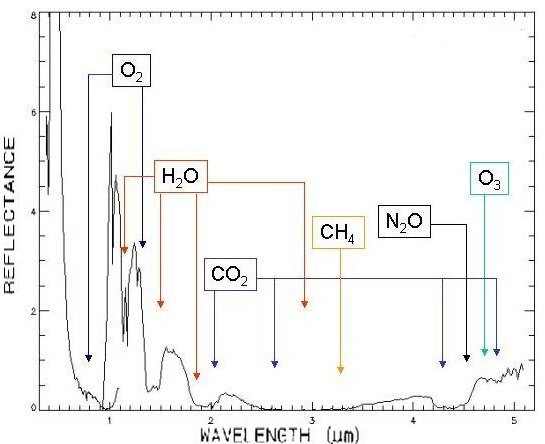
\includegraphics[width=0.45\textwidth]{figs/1.jpg}
 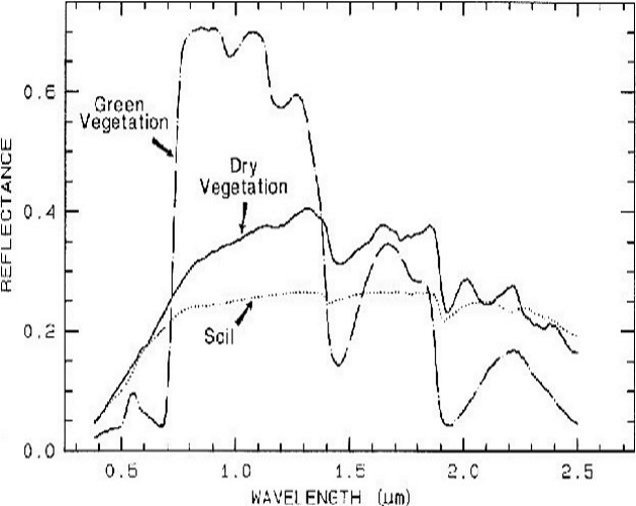
\includegraphics[width=0.45\textwidth]{figs/2.jpg}
\caption{\footnotesize (i) Mars Express record of Earth
spectrum on the visible, (ii) The vegetation spectral signature.}
\label{1}
\end{center}
\end{figure}





\subsubsection*{The Earthshine as a Tool to the Study of other Earth-like
Systems}

The observation of the spectrum of {\it Moon Earthshine}, \ie the reflection of
the Earth's light on the non-sunlit Moon, allows one to observe the
Earth as any distant planet, and to perform studies on the detectibility of
biomarkers ({\it e.g.} VRE) in its spectrum. Extracting the Earth albedo from
the Earthshine spectrum requires the measurement of moonlight spectra (lit side
of the moon) and the Earthshine spectra (unlit portion of the moon) in the
visible wavelength \citep{woolf_etal02} (see Fig. \ref{2}).



\begin{figure}[h]
\centering
 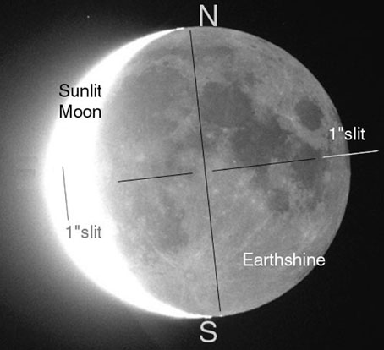
\includegraphics[scale=0.45]{figs/4.png}
 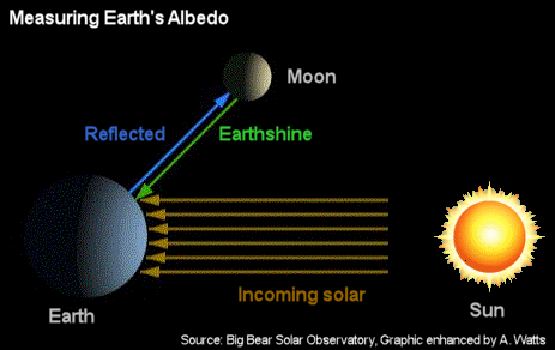
\includegraphics[scale=0.45]{figs/3.png}
\caption{\footnotesize (i) Moon's Earthshine and the schematic illustration of
the dark and bright side of the moon, (ii) Schematic illustration of the
sunlight reflected from the the Earth.}
\label{2}
\end{figure}


The spectrum of the light reflected by the planet, when normalized to the Sun
(parent star spectrum), gives the planet reflectance spectrum revealing its
atmospheric and ground color (if this is visible by a transparent
atmosphere). Quantitatively, the Earth spectrum from the Earthshine depends on
the following
variables:
\begin{itemize}
 \item the Sun spectrum as seen from outside of Earth's atmosphere, $S(\lambda)$,
\item  the Earth's atmospheric transmittance, $AT(\lambda)$,
\item the moonlight (sunlight reflected by the Moon's surface), $MS(\lambda)$,
\item the earthshine, $ES(\lambda)$,
\item the lunar reflectance, $MS(\lambda)$,
\item the Earth's reflectance, $ER(\lambda)$.
\end{itemize}

So we can write
$$ MS(\lambda) = S(\lambda) \times MR(\lambda) \times AT(\lambda) \times g_1,$$
and
$$ ES(\lambda) = S(\lambda) \times ER(\lambda) \times MR(\lambda) \times
AT(\lambda) \times g_2.$$

The Earth's reflectance is given by the ratio of the two equations,
\begin{equation}
 ER(\lambda) = \frac{ES(\lambda) g_1}{MS(\lambda) g_2},
\label{skyy}
\end{equation}
where $EM(\lambda)$ and $MS(\lambda)$ should be recorded simultaneously to avoid
airmass variation, and $g_1, g_2$ are geometric factors related to the position
of Sun, Moon and Earth, and they can be set to unity. 


The {\it vegetation red edge} is extracted from $ER(\lambda)$,
\begin{equation}
 VRE = \frac{r_I-r_R}{r_R},
\label{vge}
\end{equation}
where $r_I$ and $r_R$ are the near  infrared and red reflectance integrated over
the spectral domains ($\sim$ 10 nm width) \cite{arnold_etal07}
\cite{arnold_etal02} \cite{writeup}.


